%%%%%%%%%%%%%%%%%%%%%%%%%%%%%%%%%%%%%%%%%%%%%%%%%%%%%%%%%%%%%%%%%%%%%%%%%%%%
% AGUJournalTemplate.tex: this template file is for articles formatted with LaTeX
%
% This file includes commands and instructions
% given in the order necessary to produce a final output that will
% satisfy AGU requirements, including customized APA reference formatting.
%
% You may copy this file and give it your
% article name, and enter your text.
%
%
% Step 1: Set the \documentclass
%
%

%% To submit your paper:
\documentclass[draft]{agujournal2019}
\usepackage{url} %this package should fix any errors with URLs in refs.
\usepackage{lineno}
\usepackage[inline]{trackchanges} %for better track changes. finalnew option will compile document with changes incorporated.
\usepackage{soul}
\linenumbers
%%%%%%%
% As of 2018 we recommend use of the TrackChanges package to mark revisions.
% The trackchanges package adds five new LaTeX commands:
%
%  \note[editor]{The note}
%  \annote[editor]{Text to annotate}{The note}
%  \add[editor]{Text to add}
%  \remove[editor]{Text to remove}
%  \change[editor]{Text to remove}{Text to add}
%
% complete documentation is here: http://trackchanges.sourceforge.net/
%%%%%%%

\draftfalse

%% Enter journal name below.
%% Choose from this list of Journals:
%
% JGR: Atmospheres
% JGR: Biogeosciences
% JGR: Earth Surface
% JGR: Oceans
% JGR: Planets
% JGR: Solid Earth
% JGR: Space Physics
% Global Biogeochemical Cycles
% Geophysical Research Letters
% Paleoceanography and Paleoclimatology
% Radio Science
% Reviews of Geophysics
% Tectonics
% Space Weather
% Water Resources Research
% Geochemistry, Geophysics, Geosystems
% Journal of Advances in Modeling Earth Systems (JAMES)
% Earth's Future
% Earth and Space Science
% Geohealth
%
% ie, \journalname{Water Resources Research}

\journalname{Geophysical Review Letters}


\newcommand{\markred}[1]{\textcolor{red}{#1}}
%\newcommand{\markcyan}[1]{\textcolor{cyan}{#1}}
\newcommand{\markblue}[1]{\textcolor{blue}{#1}}
%\newcommand{\markgreen}[1]{\textcolor{magenta}{#1}}


\begin{document}

%% ------------------------------------------------------------------------ %%
%  Title
%
% (A title should be specific, informative, and brief. Use
% abbreviations only if they are defined in the abstract. Titles that
% start with general keywords then specific terms are optimized in
% searches)
%
%% ------------------------------------------------------------------------ %%

% Example: \title{This is a test title}

\title{Local lydraulic conductivity in heterogeneous porous media}

%% ------------------------------------------------------------------------ %%
%
%  AUTHORS AND AFFILIATIONS
%
%% ------------------------------------------------------------------------ %%

% Authors are individuals who have significantly contributed to the
% research and preparation of the article. Group authors are allowed, if
% each author in the group is separately identified in an appendix.)

% List authors by first name or initial followed by last name and
% separated by commas. Use \affil{} to number affiliations, and
% \thanks{} for author notes.
% Additional author notes should be indicated with \thanks{} (for
% example, for current addresses).

% Example: \authors{A. B. Author\affil{1}\thanks{Current address, Antartica}, B. C. Author\affil{2,3}, and D. E.
% Author\affil{3,4}\thanks{Also funded by Monsanto.}}

\authors{Quirine Krol \affil{1}, Itzhak Fouxon \affil{1,2}, Pascal Corso \affil{1}, Markus Holzner \affil{1,2,3,4}}



\affiliation{1}{ETH Zurich, Stefano Franscini-Platz 5, 8093 Zurich, Switzerland}
\affiliation{2}{Department of Computational Science and Engineering, Yonsei University, Seoul 120-749, South Korea}
\affiliation{3}{Swiss Federal Institute for Water Science and Technology EAWAG}
\affiliation{4}{Swiss Federal Institute for Forest, Snow and Landscape Research WSL}


%(repeat as many times as is necessary)

%% Corresponding Author:
% Corresponding author mailing address and e-mail address:

% (include name and email addresses of the corresponding author.  More
% than one corresponding author is allowed in this LaTeX file and for
% publication; but only one corresponding author is allowed in our
% editorial system.)

% Example: \correspondingauthor{First and Last Name}{email@address.edu}

\correspondingauthor{Markus Holzner}{holzner@wsl.ch}

%% Keypoints, final entry on title page.

%  List up to three key points (at least one is required)
%  Key Points summarize the main points and conclusions of the article
%  Each must be 140 characters or fewer with no special characters or punctuation and must be complete sentences

% Example:
% \begin{keypoints}
% \item	List up to three key points (at least one is required)
% \item	Key Points summarize the main points and conclusions of the article
% \item	Each must be 140 characters or fewer with no special characters or punctuation and must be complete sentences
% \end{keypoints}

\begin{keypoints}
\item enter point 1 here
\item enter point 2 here
\item enter point 3 here
\end{keypoints}

%% ------------------------------------------------------------------------ %%
%
%  ABSTRACT and PLAIN LANGUAGE SUMMARY
%
% A good Abstract will begin with a short description of the problem
% being addressed, briefly describe the new data or analyses, then
% briefly states the main conclusion(s) and how they are supported and
% uncertainties.

% The Plain Language Summary should be written for a broad audience,
% including journalists and the science-interested public, that will not have 
% a background in your field.
%
% A Plain Language Summary is required in GRL, JGR: Planets, JGR: Biogeosciences,
% JGR: Oceans, G-Cubed, Reviews of Geophysics, and JAMES.
% see http://sharingscience.agu.org/creating-plain-language-summary/)
%
%% ------------------------------------------------------------------------ %%

%% \begin{abstract} starts the second page

\begin{abstract}
[ Resolving local velocities for laminar flow in porous media is essential to transport processes. Using direct numerical simulations to solve the Navier-Stokes equations is computationally costly for statistical representative volumes. Pore network models allow for much faster solutions and resolve much larger domains. However, the pore network architecture and constitutive model for the hydraulic conductivity heavily influence the permeability and the quality of local velocity predictions. Here, we investigate the validity of a commonly used constitutive law. We start by generating three three-dimensional artificial geometries representing porous media. In this way we can control the geometrical parameters, such as the porosity and the averaged interface area. As a benchmark, we use high fidelity numerical simulations of the Navier-Stokes equations to resolve the pressure and velocity field for laminar flow in the pore-space of the artificial geometries. We propose a new definition for pores based on iso-pressure surfaces and topology changes that enables us to measure the local hydraulic resistance. We show that it can be over-estimated up to two orders of magnitude. We propose a new constitutive model that is based on the geometry of iso-pressure surfaces. This model shows that the sphericity of iso-pressure surfaces is key to predict the local hydraulic resistances of heterogeneous porous media more reliable. The distributions of local resistances and effective pore lengths show an interesting pathway to new statistical network representations of laminar flow in porous media.]
\end{abstract}

\section*{Plain Language Summary}
[ enter your Plain Language Summary here or delete this section]


%% ------------------------------------------------------------------------ %%
%
%  TEXT
%
%% ------------------------------------------------------------------------ %%

%%% Suggested section heads:
\section{Introduction}


\begin{itemize}
	\item general problem description long standing problem 
	\item solution at the darcy scale
	\item reduction of information by pore network models, review Review of pore network modelling of porous media: Experimental characterisations, network constructions and applications to reactive transport
	\item definition of pores and channels are not unique. 
	\item 
\end{itemize}

The goal of this study is to perform Direct Numerical Simulations (DNS) that solve the Navier-Stokes equations in heterogenous porous media. The boundary conditions are chosen such that Re number is chosen within the Stokes regime $Re\ll1$. These simulations enables us to know the locally the velocity $\mathbf{u}$ and the local pressure field $p$. We propose a new definition of local pores for which we can measure the local pressure drop and the internal resistance of the porous media. 



\section{Theoretical Background}
\subsection{Static Navier stokes equations in porous media}
We assume that for low Reynolds number, incompressible flow in a porous media, the local flow can be described by the Navier-Stokes equations. 
\begin{equation}\label{eq:stokes_local}
	\mathbf{\nabla} p = - \nu\mathbf{\nabla}^2 \mathbf{u}\,,\,\mathbf{\nabla}\cdot\mathbf{u}=0
	\end{equation}
with pressure $p$ and velocity $\mathbf{u}$ and kinemetic viscosity $\nu$. 
For a volume $V$ in a porous media, enclosed by surface $\partial V$ given by two isopressure surfaces $S_{p_1}$ and $S_{p_2}$ and a remaining a porous media domain $\Gamma$, we can write down the integral form of the Navier-Stokes equations


\begin{equation}\label{eq:stokes_dissipation}
\int_V \left(\mathbf{u}\cdot\mathbf{\nabla} p-\nu \mathbf{u}\cdot\mathbf{\nabla}^2 \mathbf{u}\right) dV 
= \int_{\partial V}  p\,\mathbf{u}\cdot\mathbf{n}\,dS+\eta \int_{\partial V} \mathbf{u} (\mathbf{\nabla} \mathbf{u})\cdot\mathbf{n}\,dS-\eta \int_{V} (\mathbf{\nabla}\, \mathbf{u})^2 dV=0
\end{equation}

Given that at the porous media boundary domain $\Gamma$ we have a no-slip condition $\mathbf{u}=0$ we can write \markred{check signs}

\begin{equation}\label{eq:pressuredrop}
	Q \Delta p = -\eta\int_{S_{p_1}+S_{p_2}} \mathbf{u} (\mathbf{\nabla} \mathbf{u})\cdot\mathbf{n}\,dS -\eta \int_V (\mathbf{\nabla}\, \mathbf{u})^2 dV,
\end{equation}


with the total flux defined by 

\begin{equation}
	Q=\int \mathbf{u}\cdot\mathbf{n}\, dS.
\end{equation}


%???? We observe that $dS_k=dS \nabla_k p/|\nabla p|$.


\subsection{Hagen-Poiseuille Flow} 

For a specific geometry of a pipe with Radius $R$ and length $L$, the second term from Eq.\ref{eq:pressuredrop} of the right-hand-side vanishes by symmetry considerations (i.e. the viscous work is zero). The exact solution for the local velocity can be obtained and is given by 
\begin{equation}\label{eq:poiseuille}
v(r)=U \left(1-\frac{r^2}{R^2}\right),
\end{equation}
with $U$ the maximal velocity. The flux $Q$, pressure gradient and the hydraulic resistance $\mathcal{R}:=\Delta p/Q$ can be simply written by
\begin{equation}
	Q=\frac{\pi R^2 U}{2}\,,\,\frac{\Delta p}{L}=-\frac{4\eta U}{R^2}\, , \, \mathcal{R}_{\rm{hp}}= \frac{\eta L}{\pi^2 R^4}
\end{equation}


\subsection{Pore identification}

\begin{centering}
\begin{figure}[t!]\label{fig:isop_surfaces}
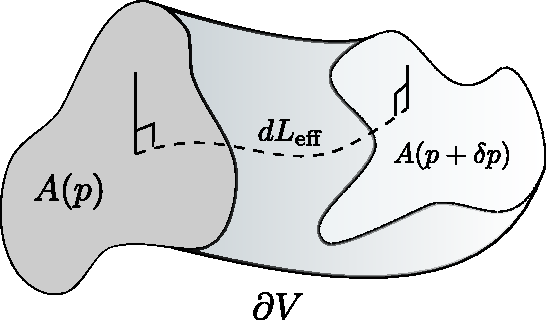
\includegraphics[height=4cm]{figures/isopressure_surfaces.pdf}~~~~
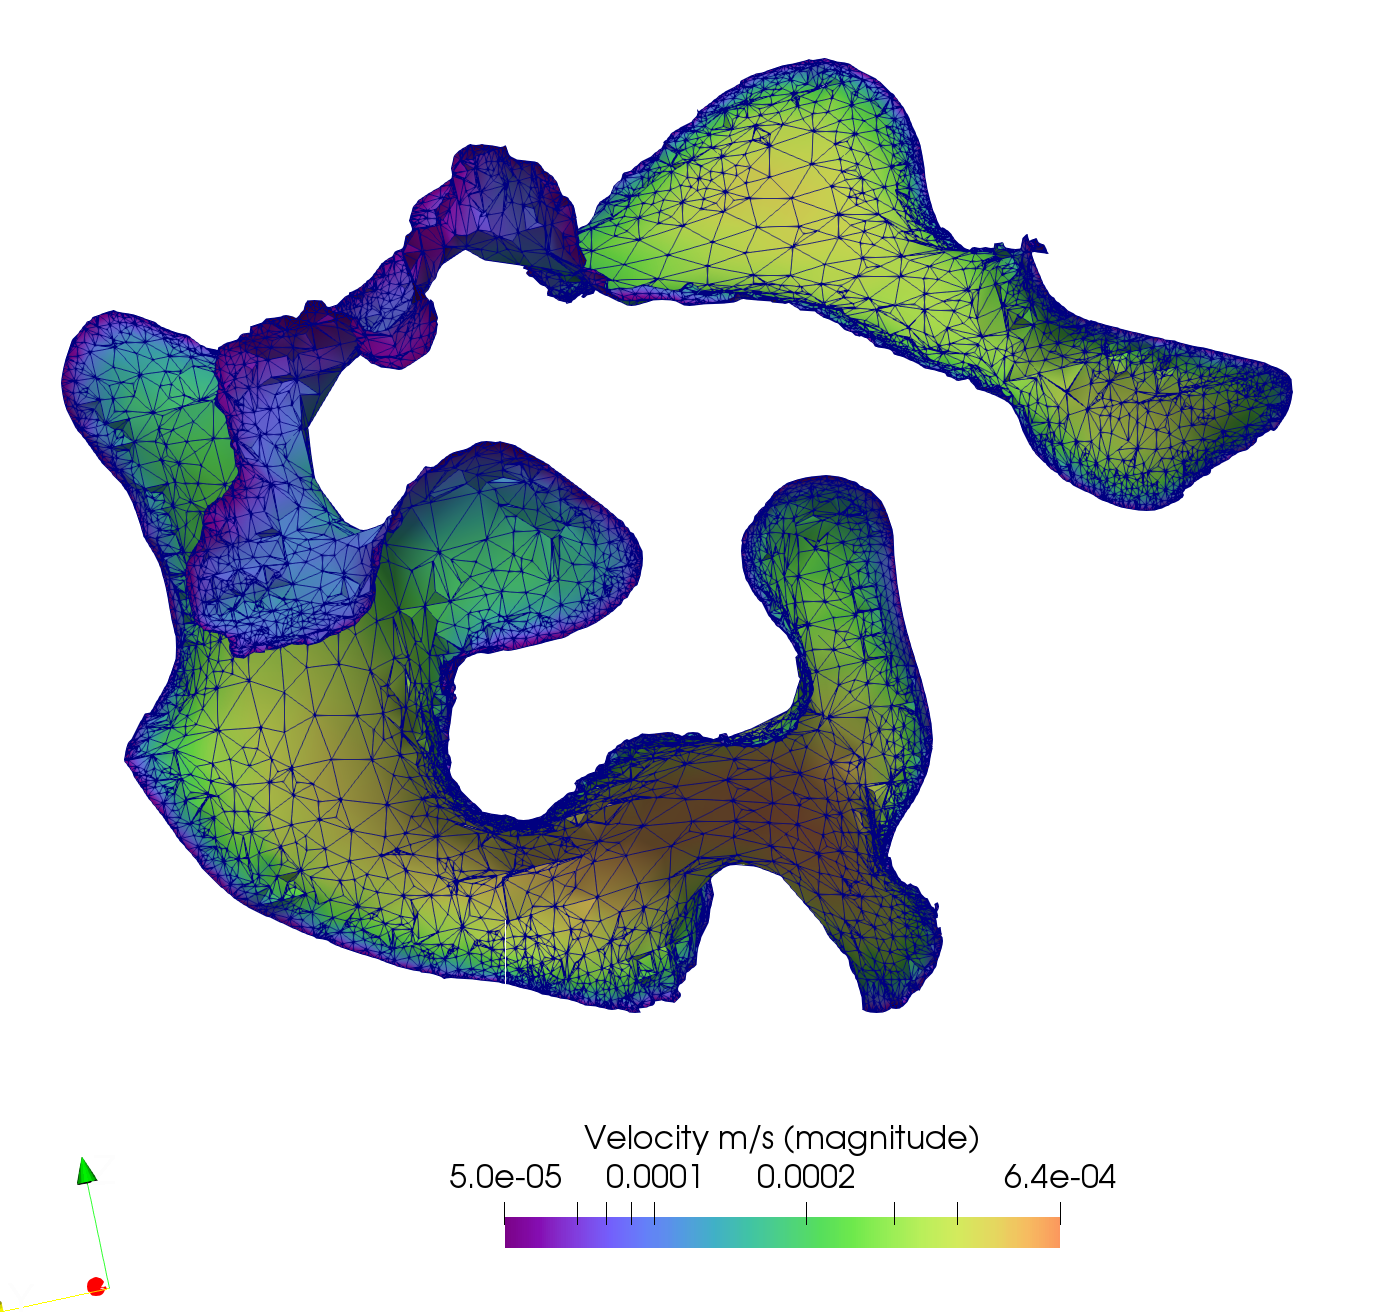
\includegraphics[height=5cm]{figures/iso_segmentation_example.png}
\caption{A visualization a volume enclosed by iso pressure surfaces and the boundary of the geometry.}
\end{figure}
\end{centering}
For porous media with arbitrary geometry, there is no standard definition for individual pores that collectively build up the pore space in a porous media. A law for local the hydraulic resistance between two iso-pressure surfaces such as for the Hagen-Poiseuille case is still missing, since one cannot apply the symmetry argument to solve the Navier-Stokes equations exactly. To relate to the concept of a network of pores with certain hydraulic resistances a definition of a pore is indispensable. Most pore-network models represent pores by junctions without an internal pressure drop, and the connections between the junctions are represented by a channel, given a certain hydraulic resistance. Here we introduce the notion of disconnected iso-pressure surfaces $\mathcal{S}_i(p)$ for a given pressure value $p$.
It is useful to observe that this consideration works for any fluid tube bounded by iso-pressure surfaces and iso-pressure surface of velocity magnitude at which velocity is (approximately) zero. Considering completely saturated conditions the boundary terms of Eq.~\ref{eq:stokes_dissipation} will be drop when multiple pores are added (meaning $\mathbf{n}\rightarrow -\mathbf{n}$). Therefore Eq.~\ref{eq:stokes_dissipation} intrinsically will only evaluate

\begin{equation}\label{eq:pore_based_energy_dissipation}
Q \Delta p=\eta \int (\nabla \mathbf{u})^2 dV,
\end{equation}

When we consider a decomposition of the velocity vector  $\mathbf{u} = u_p \mathbf{\hat{p}} + u_r \mathbf{\hat{r}}$ with $\mathbf{\hat{p}} =\mathbf{ \nabla}p/|\mathbf{ \nabla}p|$. For HP flow $\mathbf{u}$ is parallel to the pressure gradient, for which in simple geometries exact solutions can be derived. In the following we will assume that the most important contributions to the dissipation tensor $\nabla_i u_j$ is given by the assumption that $u_r \ll u_p $ yielding 

\begin{equation}\label{eq:reduced_dissipation_tensor}
\left|\nabla_i u_j\right|^2 \approx  \left|\nabla_r u_p\right|^2 + \left|\nabla_p u_p\right|^2 .
\end{equation}

Here the first term is much more important since the velocity-velocity correlation length in the longitudinal direction is usually much larger than the average pore size. When we consider the dissipation of an infinitesimal enclosed volume $dV$ defined by $\mathcal{S}_i,\mathcal{S}_{i+1}$ and their respective areas $A_i, A_{i+1}$, separated by average distance $dx$ we can estimate the first term of Eq.~\ref{eq:reduced_dissipation_tensor} analogous as done by \cite{mortensen_reexamination_2005} with
\begin{equation}
	\left|\nabla_r u_p\right|^2 = \left(\alpha_0+\alpha_1\,\gamma^{-2}\right)\frac{ Q^2}{A^3}~~~ \rm{with}~~~ ,
\end{equation}
with sphericity parameter $\gamma^{-1} = \mathcal{L}/\sqrt{ 4\pi A(p)}$ with perimeter $\mathcal{L} = \int_{\partial \mathcal{S}_i}dl$. The sphericity parameter is inversely related to the compactness factor $\gamma^{-2}\sim \mathcal{C} $in \cite{mortensen_reexamination_2005}. The coefficient $a$ and $b$ can be calculated for simple shapes of the iso-pressure surfaces, such as squares, triangles, or a perturbation of a sphere by spherical harmonics \citeA{mortensen_reexamination_2005}. For heterogeneous media the class of shapes are generally unknown. For the second, longitudinal term, we can assume that the total flux $Q$ remains constant for $p\rightarrow p+dp$, and the change of velocity is caused by a change in crossectional area $A_i$
\begin{equation}
	\left|\nabla_p u_p\right|^2 = \alpha_2  \frac{Q^2}{A^4}\left|\frac{\partial A}{\partial x }\right|^2,
\end{equation}
with unknown $\alpha_2$. When we combine the two expressions we obtain, for infinitesimal pressure difference $d p$ and corresponding $dV = A dl_{\rm{eff}}$

\begin{equation}\label{eq:infi_dp}
	dp = \frac{Q}{A^2} f\left(\alpha_i,\mathcal{S}(p)\right) dx= \frac{Q}{A^2}\left(\alpha_0+\alpha_1\gamma^{-2} + \alpha_2 \frac{1}{A}\left|\frac{\partial A}{\partial x }\right|^2\right)\,dx
\end{equation}

The total pressure gradient along a full pore is then given by 

\begin{equation}
	\frac{\Delta p}{L_{\rm{eff}}} =  Q \frac{1}{L_{\rm{eff}}}\int^{L_{\rm{eff}}}_{0}\frac{1}{A^2}f\left(\alpha_i,\mathcal{S}(p)\right)\,dx
\end{equation}

with 
\begin{equation}
	L_{\rm{eff}} = \int^{L_{\rm{eff}}}_{0} dx
\end{equation}

from which we find a expression for a model for the total hydraulic resistance 

\begin{equation}\label{eq:R_model}
	\mathcal{R}_m = \int^{L_{\rm{eff}}}_{0}\frac{1}{A^2}f\left(\alpha_i,\mathcal{S}(p)\right)\,dx
\end{equation}


\begin{figure}[t!]\label{fig:DNS}
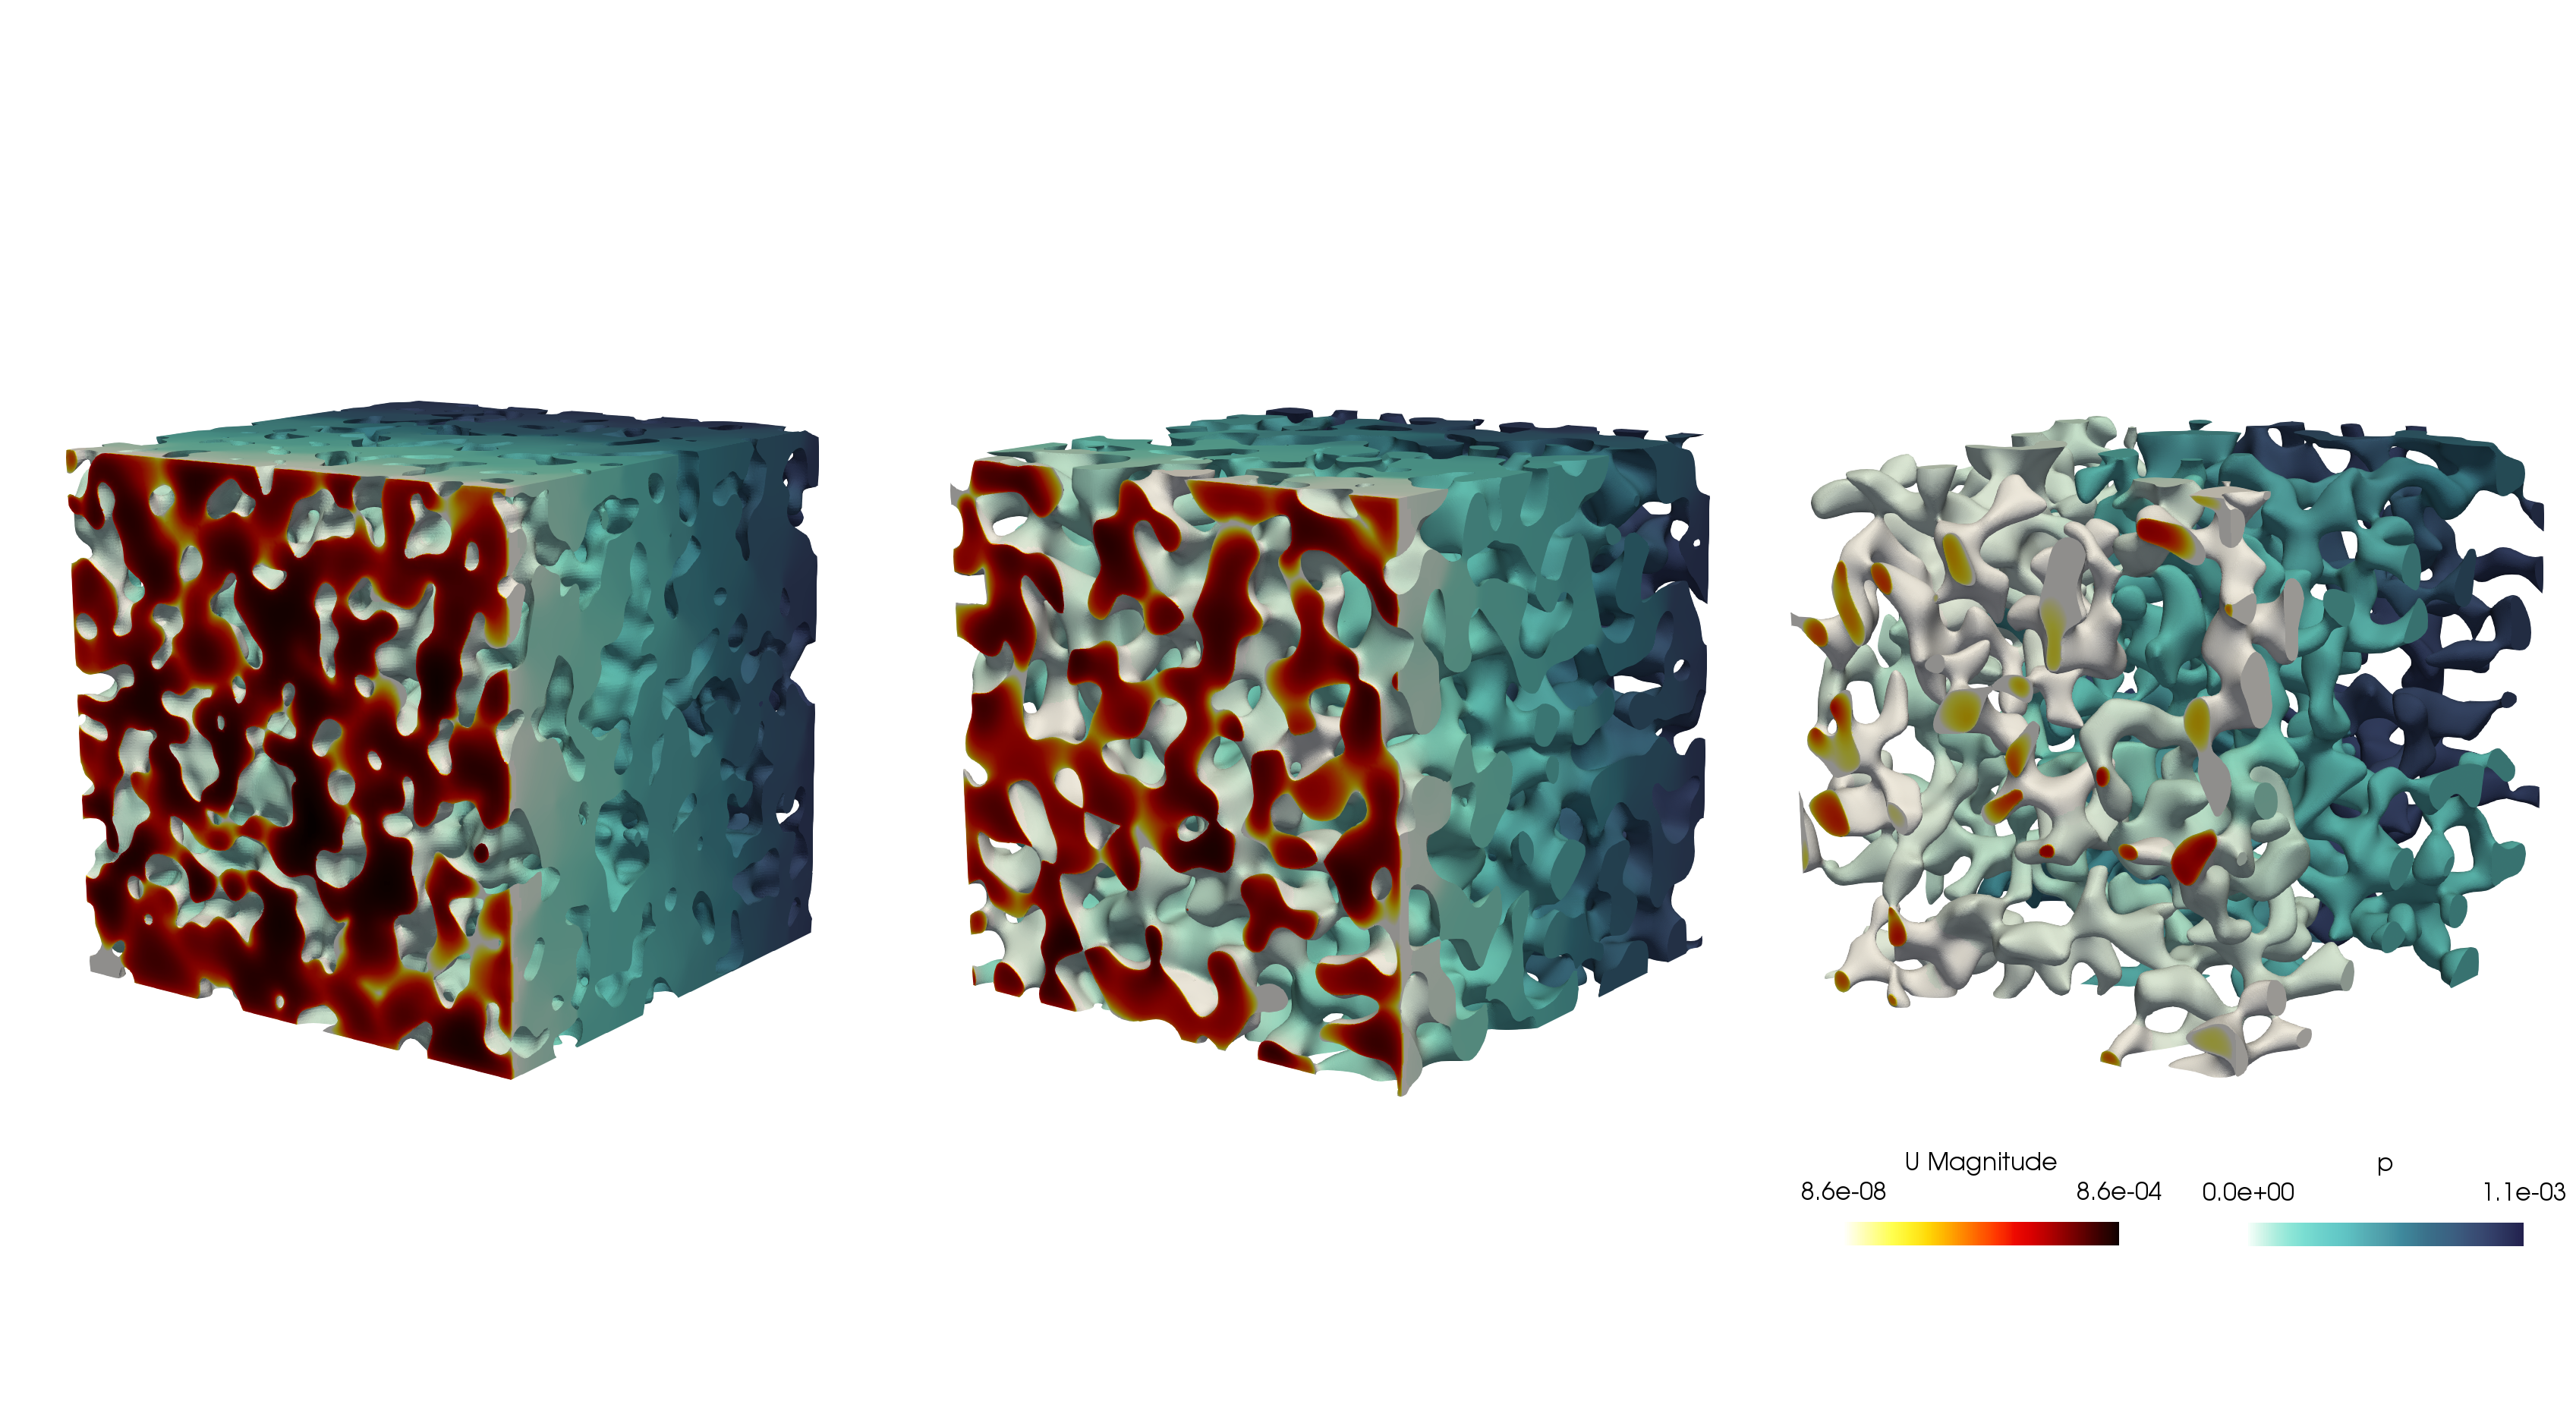
\includegraphics[height=8cm]{figures/PM_combined_surfaces_DNS.png}
\caption{A visualization of the velocity field $|u|$ and pressure field $p$ in the pore space of the three porous media used in this study.}
\end{figure}


\subsection{Methods}

\begin{figure}[htbp!]\label{fig:segmentation}
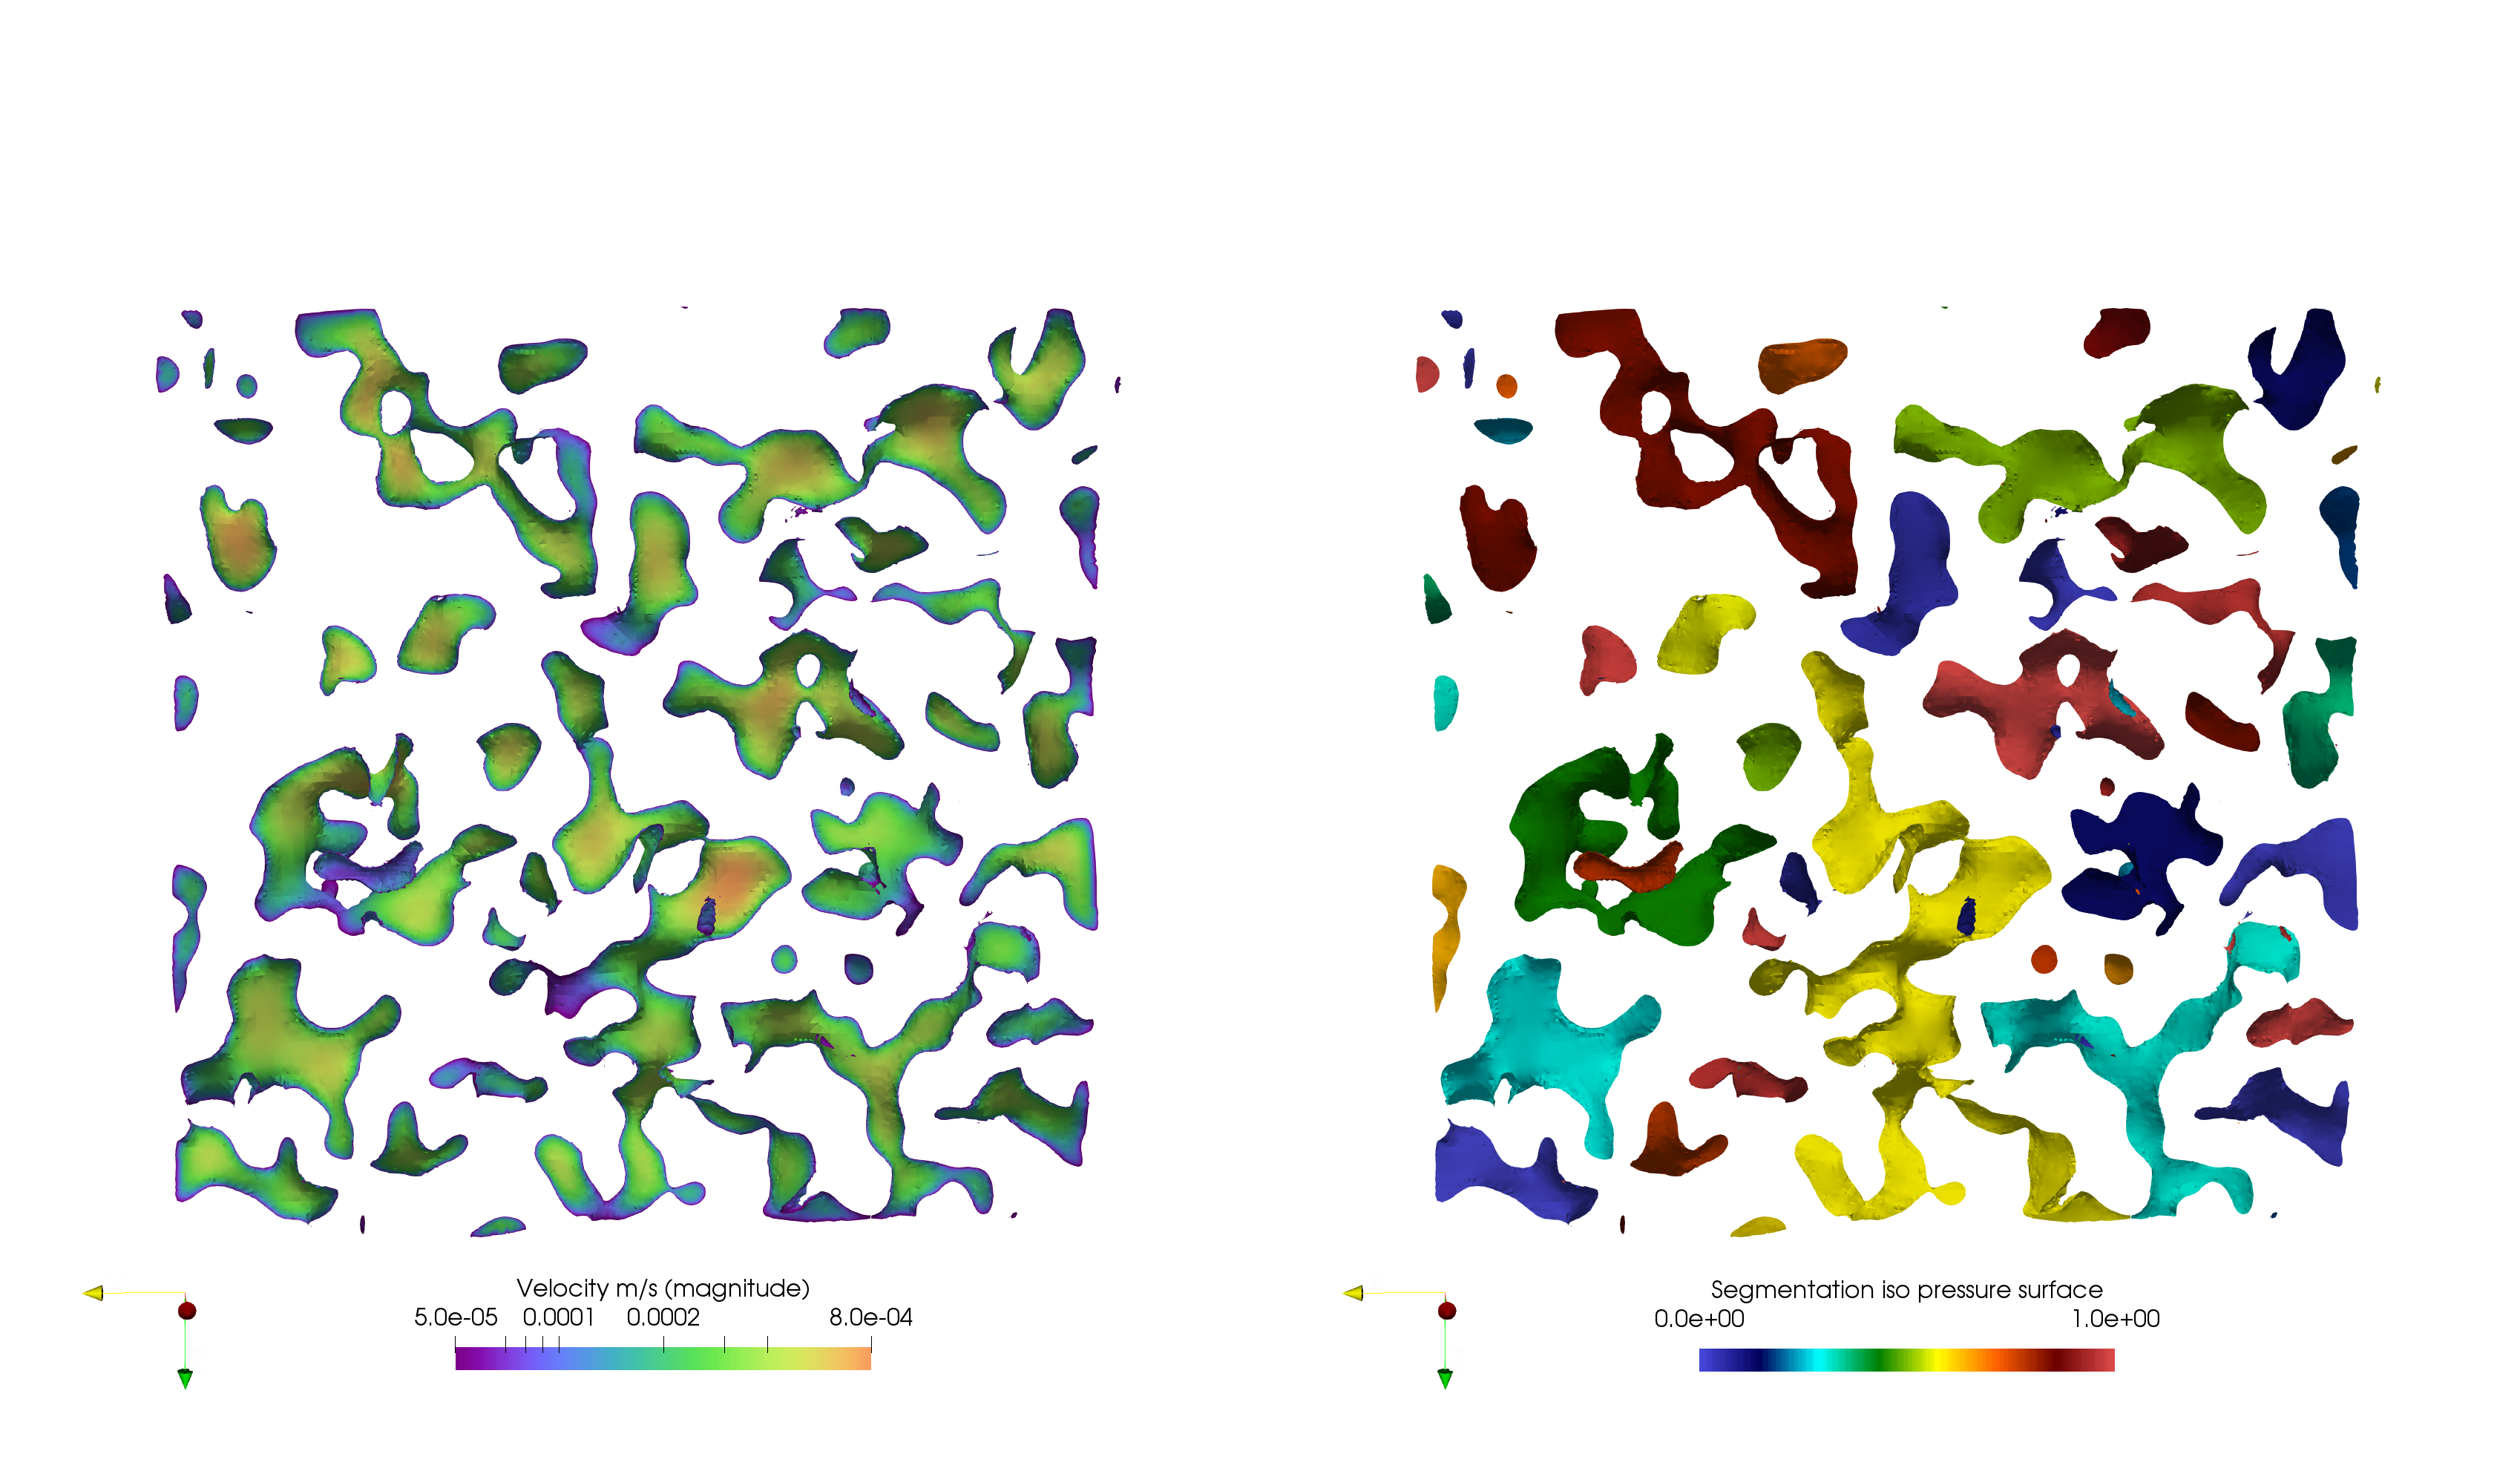
\includegraphics[height=6cm]{figures/semgentation_veloctiy_iso_p_surface.png}
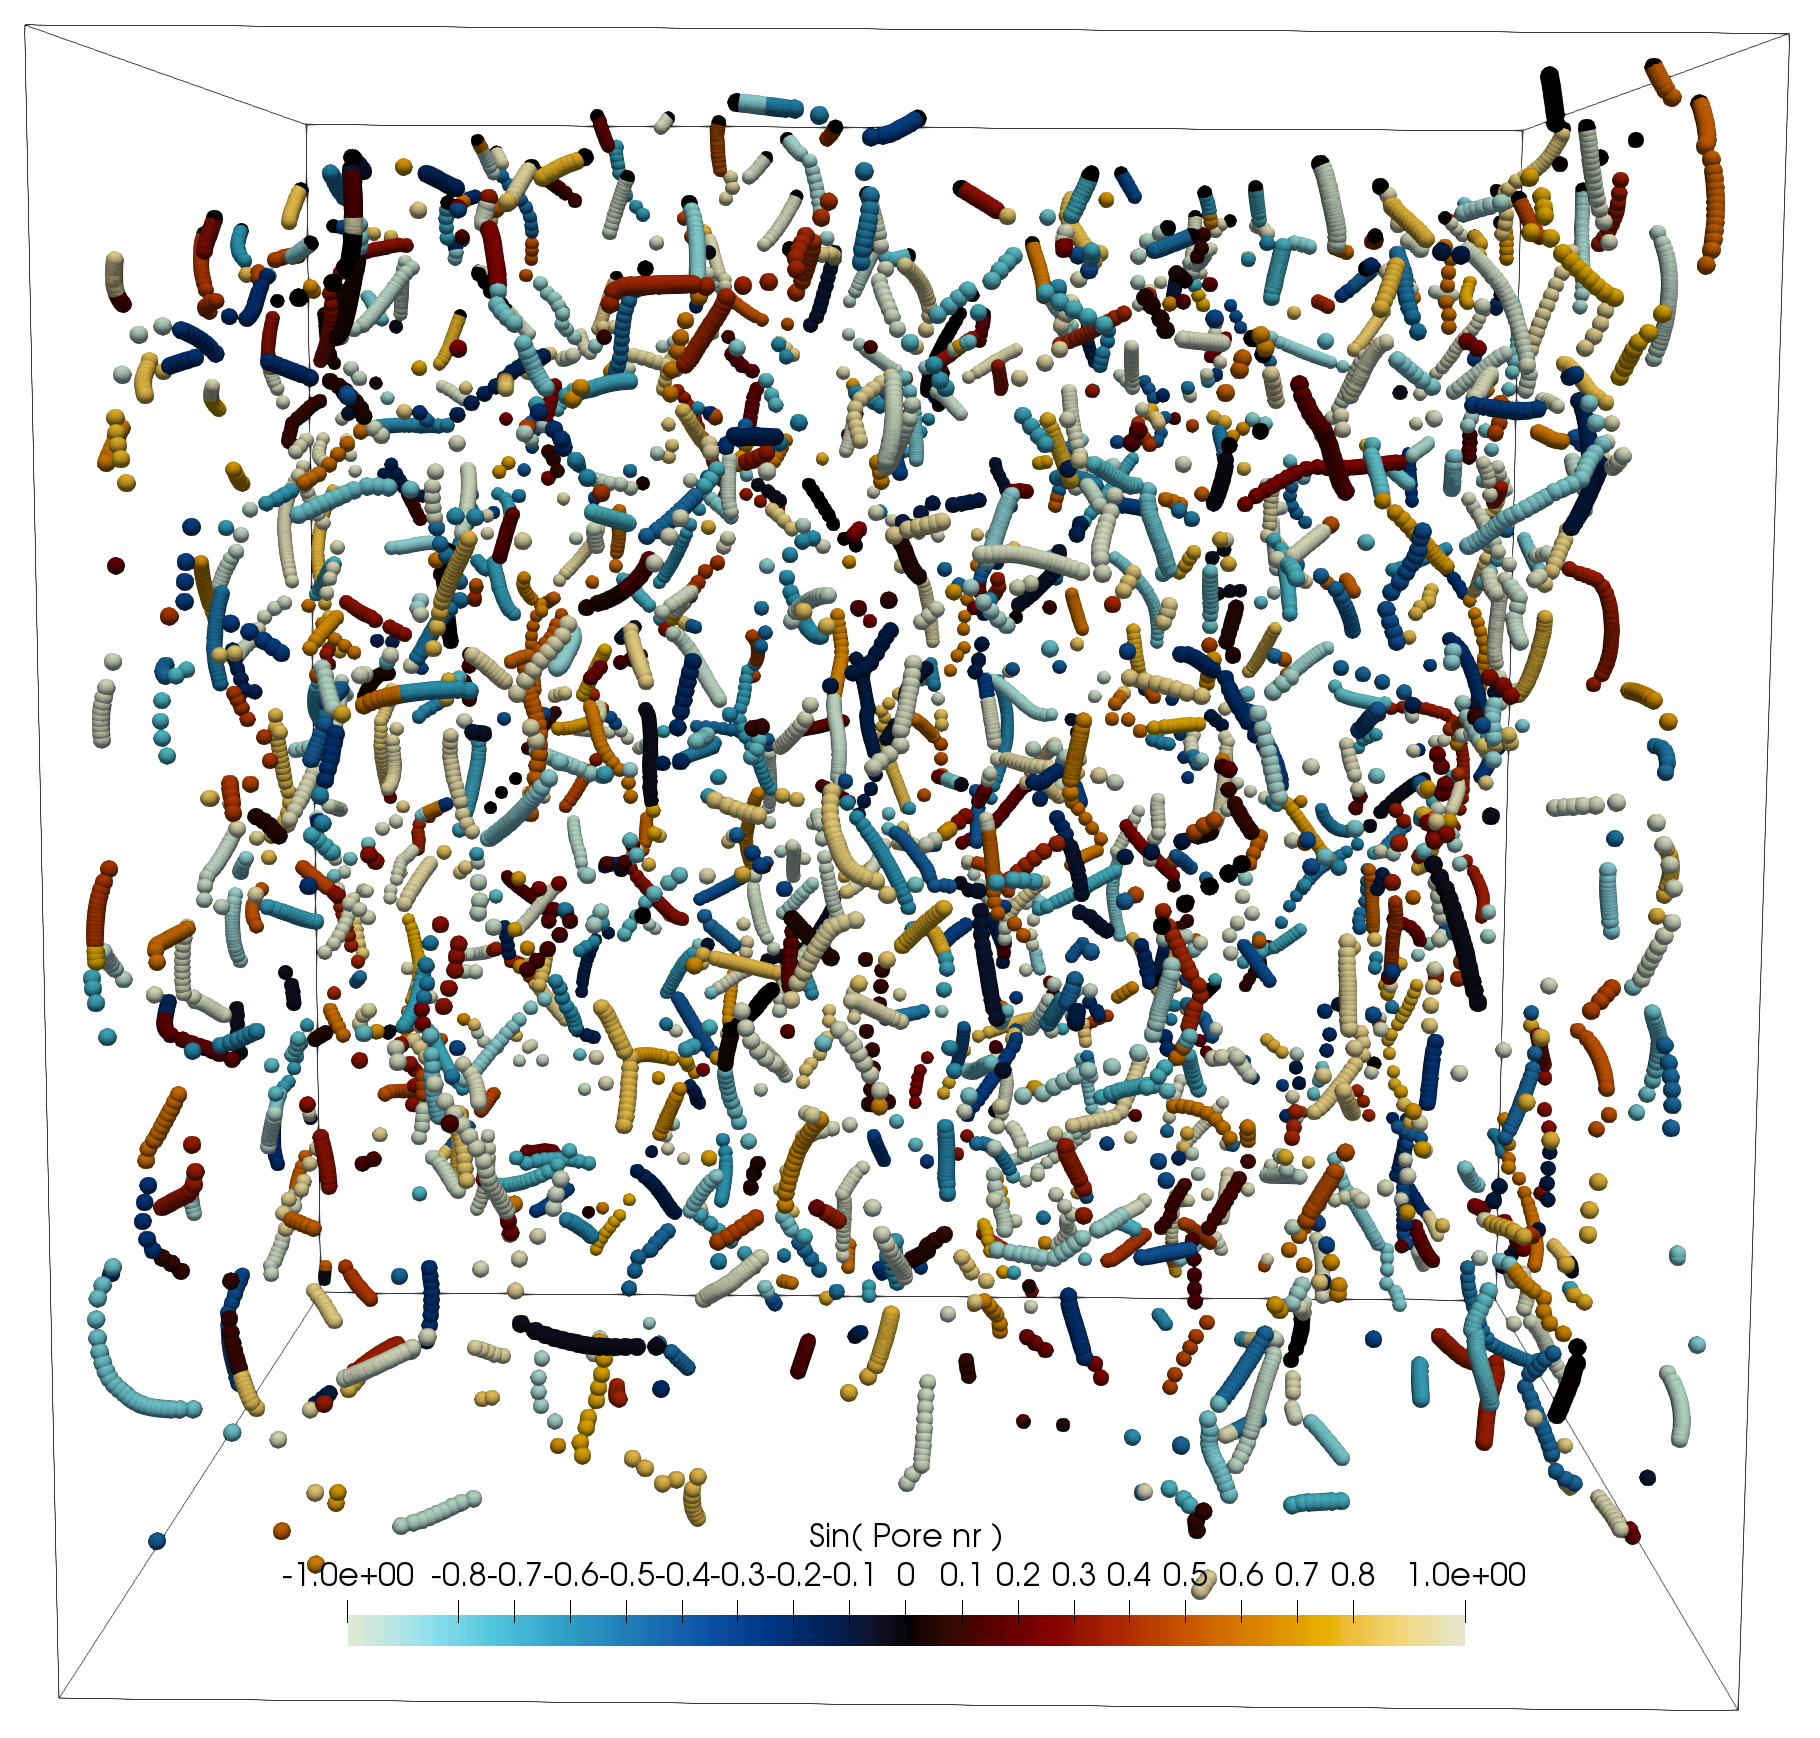
\includegraphics[height=5cm]{figures/pores_PM2.png}
\caption{Visualization of left: velocity field $|\mathbf{u}|$of an iso-pressure surface $\mathcal{S}(p)$ at pressure value $p$, middle: segmentation into iso-pressure patches  $\mathcal{S}_i(p)$, right: Pore identification throughout the porous medium. }
\end{figure}

To generate heterogeneous porous media we have used Gaussian Random Fields to generate 3 porous media. A threshold is used to define the porous media-fluid interface $\Gamma$ and its porosity. eq $0.68, .34 $ and $.16$. In Table 



These porous media are used as input for direct numerical simulations (OpenFOAM v. 4.1) \citeA{weller_tensorial_1998}  that solves the Navier-Stokes equations in the pore space. The boundary conditions are defined at the inlet $p_1$ and outlet $p_2$ and a no-slip for the porous media-fluid interface. A visualization of the three porous media an the result of the DNS is visualized in Fig.~\ref{fig:DNS}
Then a chain of VTK-based image analysis techniques \citeA{schroeder_visualization_2006,hernderson_paraview_2007} are employed to extract iso-pressure surfaces $\mathcal{S}(p)$ and enumerate the disconnected areas identifying as an iso-pressure slice $\mathcal{S}_i(p)$, part of a pore and measure its surface area $A_i(p)$, sphericity $\gamma_i(p)$, average location $\mathbf{x}_i(p)$ and average flux $Q_i(p)$. For each $\mathcal{S}_i(p)$ its closest neighbor $\mathcal{S}_j(p+\delta p)$ is identified by its smallest distance $d_{i,j}= \left|  \mathbf{x}_i(p)-\mathbf{x}_j(p+\delta p)\right|$. By forward integration of the first iso-pressure patches $\mathcal{S}_i(p_0)$ we identify all patches belonging to the same pore $\mathcal{P}_l(\Delta p) = \{\mathcal{S}_k(p_i)\}$. By conditioning the distances of consecutive iso pressure patches to a maximum, the ends of a pore is defined. When a splitting/merging of pores is at hand, the average position is rather sensitive, and the distance between two consecutive iso-pressure pore patches will exceed the maximum distance. Fig.~\ref{fig:segmentation} shows a visualization of the positions of the identified pores. For each $\delta p$ we can now evaluate Eq.~\ref{eq:infi_dp} and for each pore, we can evaluate Eq.~\ref{eq:R_model}. A visualization of an iso-pressure surface $\mathcal{S}(p)$ and its devision of patches is shown in Fig.\ref{fig:segmentation}. 



\section{Results} 
Fitted values for $\alpha $:

\begin{table}[htbp!]
\centering
\begin{tabular}{l|c|c|c|c}
Geometry: & porosity & spec. surface area $A/V$ &rel. pore size $ l_p/L$ & roughness $\rm{std}(H)^{-1}/L$ \\
\hline
PM1 & $0.68$ & $2.0\times10^{4}$ & $0.17$ &  $2.3\times10^{-2}$\\
PM2 & $0.34$ & $1.8\times10^{4}$ & $0.08$ &  $3.5\times10^{-2}$\\
PM3 & $0.17$ & $1.2\times10^{4}$ & $0.06$ &  $2.1\times10^{-2}$\\
\hline
Fitting parameters: & $\alpha_0$ & $\alpha_1$ & $\alpha_2$ & $R^2$  \\
\hline
PM1 & $0.26$ & $0.72$ & $4.7\times 10^{-3}$ &  $0.93$\\
PM2 & $.40$ & $0.69$ & $1.3 \times 10^{-3}$ & $0.98$ \\
PM3 & $0.98$ & $0.32$ & $0.22$ & $0.99$ \\
\end{tabular}
\caption{\label{tab:table-name}Results for fitted parameters.}
\end{table}
Note the deviations for PM3.


Renoyld numbers for these media 
\begin{equation}
	Re_{1,2} = \frac{q \sqrt{A}}{\eta}\approx 1.5 \times 10^{-5}, Re_2 \approx 8 \times 10^{-6}, Re_3 = 8 \times 10^{-7}
\end{equation}

\subsection{infinitesimal hydraulic conductivity}

\begin{figure}\label{fig:local_and_integrated}
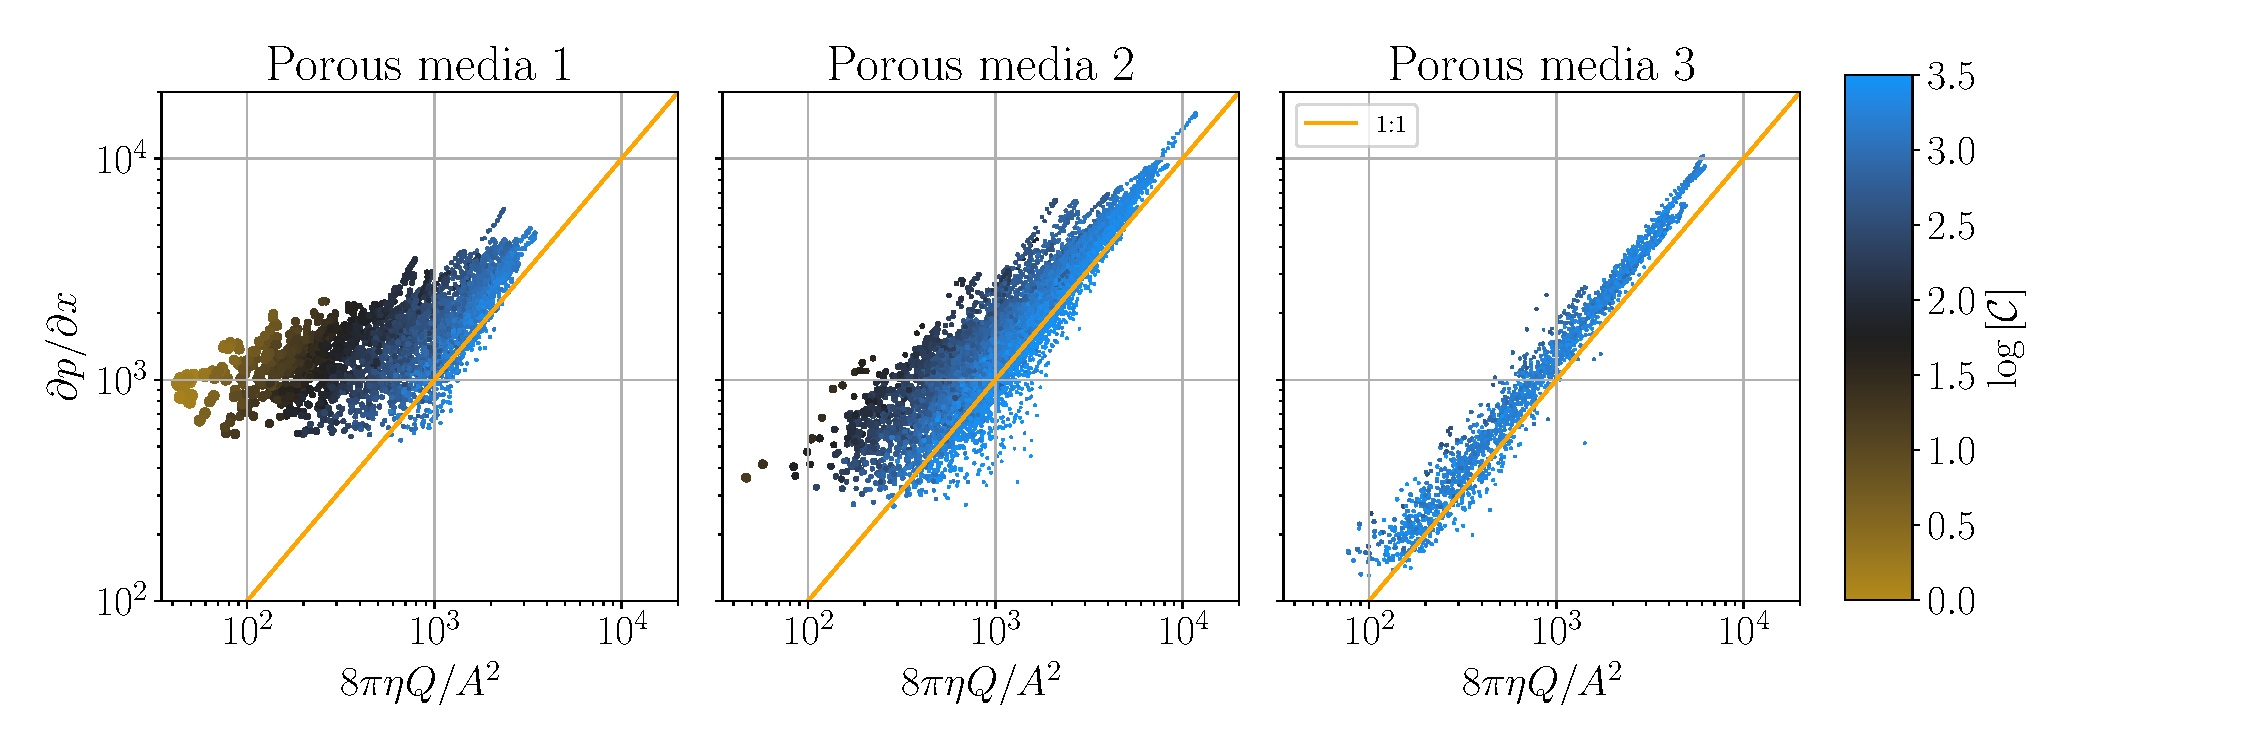
\includegraphics[height=6cm]{figures/infi_dpdx_3.pdf}
\caption{Measurements of local hydraulic conductivity for three different porous media}
\end{figure}

local model for $\alpha$

\begin{figure}\label{fig:local_and_integrated}
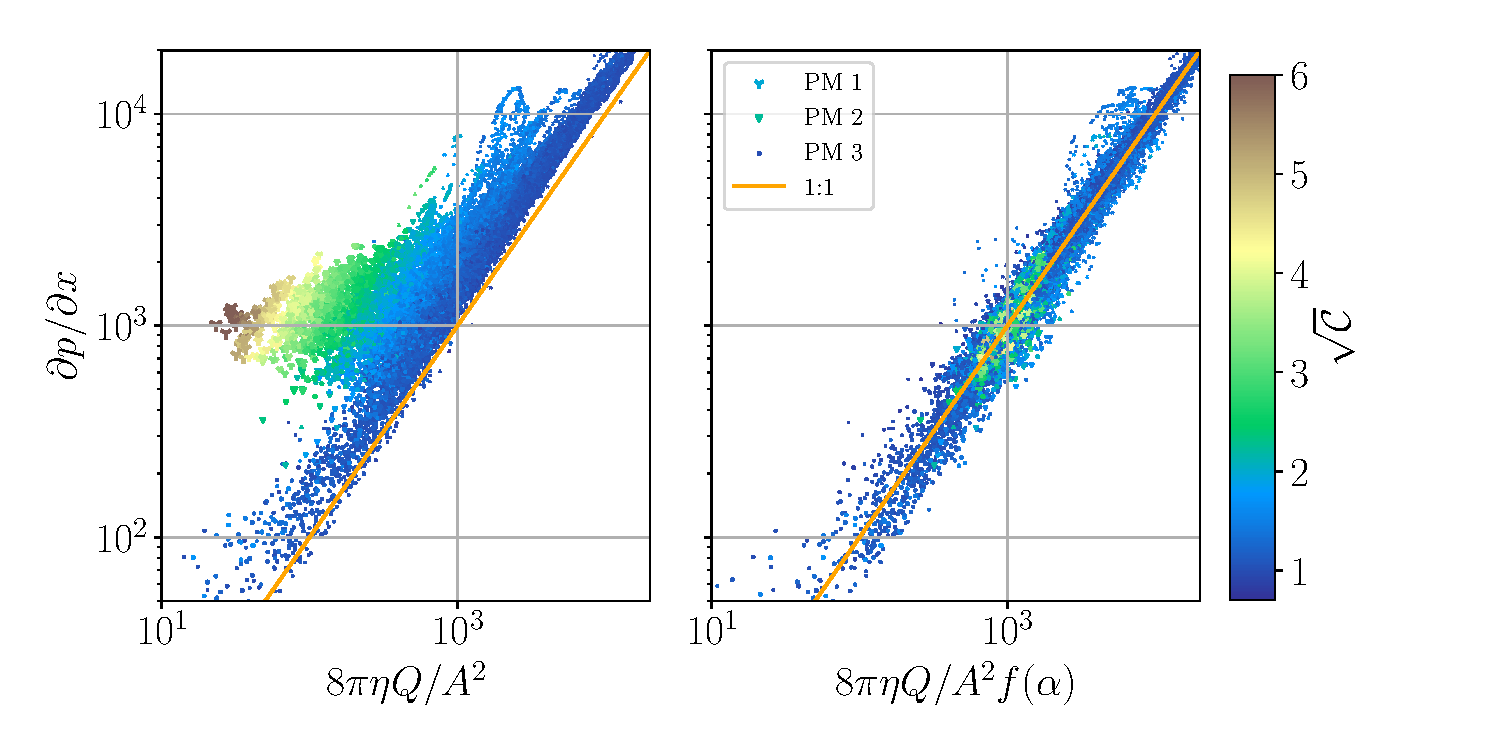
\includegraphics[height=8cm]{figures/infi_dpdx_combined.pdf}
\caption{Measurements of local hydraulic conductivity for three different porous media}
\end{figure}

as well functions in an integrable fashion

\begin{figure}\label{fig:local_and_integrated}
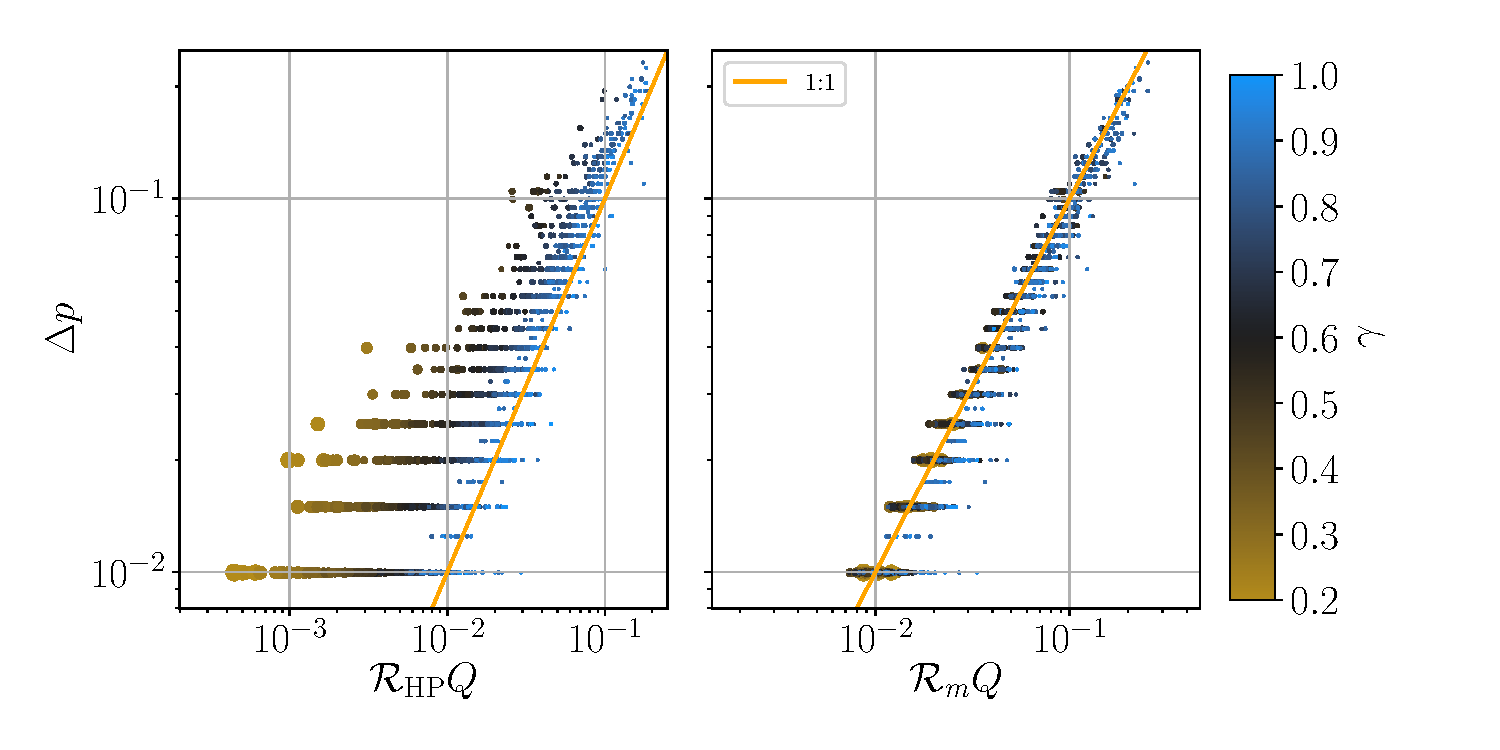
\includegraphics[height=8cm]{figures/integral_dp_combined.pdf}
\caption{Measurements of local hydraulic conductivity for three different porous media}
\end{figure}


\subsection{Integrated along pores}

\begin{figure}\label{fig:histogram_R}
\centering{
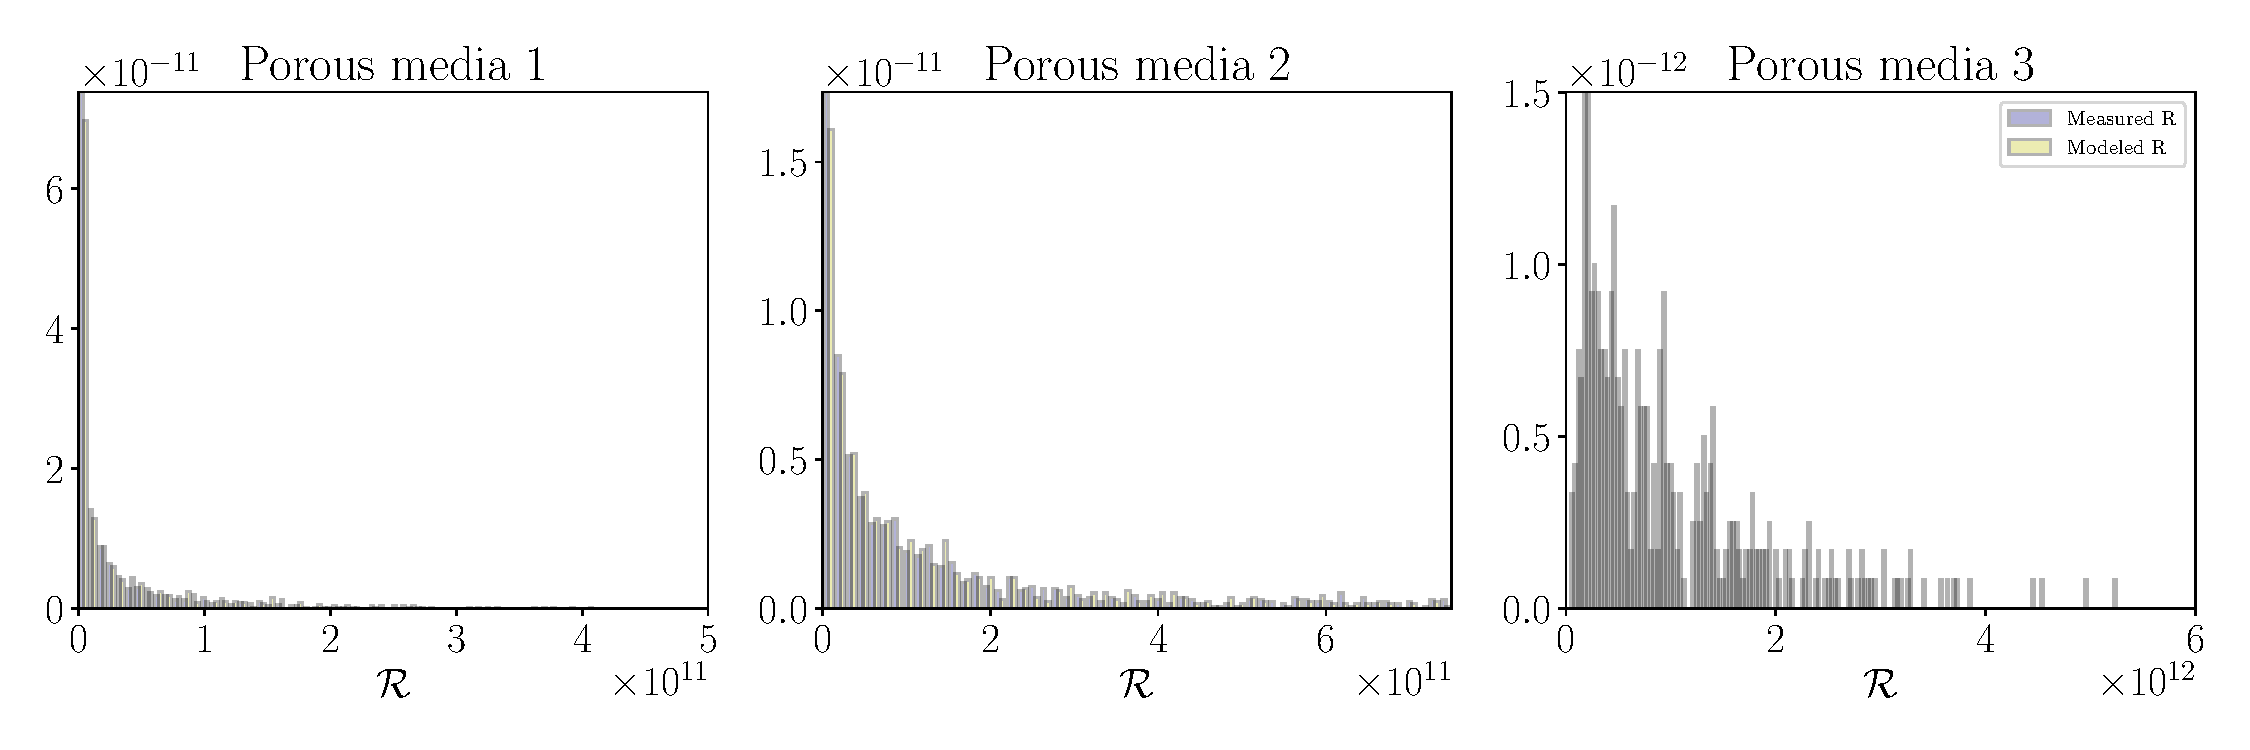
\includegraphics[height=5cm]{figures/hydrualic_conductivity_integrated_histogram.pdf}
\caption{Histogram of the measured and modeled hydraulic conductivity $\mathcal{R}$.}}
\end{figure}


\section{Discussions}

Discussion on sentivities of the method 
\begin{enumerate}
	\item Choosing $u_0$ to minimize point noise area patches of $S_i$, because of the mesh representation close to the inteface.
	\item Choosing $dx_{max}$
	\item small pores, can also have a very complex shape, since there are more topology changes to be expected when $S_i$ is highly convoluted, as indicated by high $\gamma$. for Eq.~\ref{eq:infi_dp} needs at least 2 isopressure surface patches. 
	\item sphericity values higher than $\gamma >0$
	\item Measured resistances function $f(\alpha) < 1$, is physically impossible. Here we measure a small portion that violates this physics. this is possible due to the method of cutting the iso pressure surfaces with a value $u_{min}$ leading to smaller areas. We have tried to correct for it with a factor that is calculated by the difference between the maximum $v_{max}-v_{min}$ by a linear extension of the area.  , but it is difficult to do this for very small areas since the cutoff of the area by $v_min$ is quit a significant portion. 
	\item The removal of the all the noise produced from the very fine mesh at close to the porous media interface is practically impossible, therefore, the final data has another threshold in the post processing on very small areas.   
\end{enumerate}


\section{Conclusions}
\begin{itemize}
	\item We propose a new `natural' way of defining a pore with the aim of modeling the local hydraulic conductivity that can be used in a pore-network model. By integrating isopressure surfaces from  
\end{itemize}

\section{Odd observations}
\begin{itemize}
	\item $u_s$ is relatively high when iso-pressure surfaces have a hole, (genus < 0)
\end{itemize}

%Text here ===>>>


%%

%  Numbered lines in equations:
%  To add line numbers to lines in equations,
%  \begin{linenomath*}
%  \begin{equation}
%  \end{equation}
%  \end{linenomath*}



%% Enter Figures and Tables near as possible to where they are first mentioned:
%
% DO NOT USE \psfrag or \subfigure commands.
%
% Figure captions go below the figure.
% Table titles go above tables;  other caption information
%  should be placed in last line of the table, using
% \multicolumn2l{$^a$ This is a table note.}
%
%----------------
% EXAMPLE FIGURES
%
% \begin{figure}
% \includegraphics{example.png}
% \caption{caption}
% \end{figure}
%
% Giving latex a width will help it to scale the figure properly. A simple trick is to use \textwidth. Try this if large figures run off the side of the page.
% \begin{figure}
% \noindent\includegraphics[width=\textwidth]{anothersample.png}
%\caption{caption}
%\label{pngfiguresample}
%\end{figure}
%
%
% If you get an error about an unknown bounding box, try specifying the width and height of the figure with the natwidth and natheight options. This is common when trying to add a PDF figure without pdflatex.
% \begin{figure}
% \noindent\includegraphics[natwidth=800px,natheight=600px]{samplefigure.pdf}
%\caption{caption}
%\label{pdffiguresample}
%\end{figure}
%
%
% PDFLatex does not seem to be able to process EPS figures. You may want to try the epstopdf package.
%

%
% ---------------
% EXAMPLE TABLE
%
% \begin{table}
% \caption{Time of the Transition Between Phase 1 and Phase 2$^{a}$}
% \centering
% \begin{tabular}{l c}
% \hline
%  Run  & Time (min)  \\
% \hline
%   $l1$  & 260   \\
%   $l2$  & 300   \\
%   $l3$  & 340   \\
%   $h1$  & 270   \\
%   $h2$  & 250   \\
%   $h3$  & 380   \\
%   $r1$  & 370   \\
%   $r2$  & 390   \\
% \hline
% \multicolumn{2}{l}{$^{a}$Footnote text here.}
% \end{tabular}
% \end{table}

%% SIDEWAYS FIGURE and TABLE
% AGU prefers the use of {sidewaystable} over {landscapetable} as it causes fewer problems.
%
% \begin{sidewaysfigure}
% \includegraphics[width=20pc]{figsamp}
% \caption{caption here}
% \label{newfig}
% \end{sidewaysfigure}
%
%  \begin{sidewaystable}
%  \caption{Caption here}
% \label{tab:signif_gap_clos}
%  \begin{tabular}{ccc}
% one&two&three\\
% four&five&six
%  \end{tabular}
%  \end{sidewaystable}

%% If using numbered lines, please surround equations with \begin{linenomath*}...\end{linenomath*}
%\begin{linenomath*}
%\begin{equation}
%y|{f} \sim g(m, \sigma),
%\end{equation}
%\end{linenomath*}

%%% End of body of article

%%%%%%%%%%%%%%%%%%%%%%%%%%%%%%%%
%% Optional Appendix goes here
%
% The \appendix command resets counters and redefines section heads
%
% After typing \appendix
%
%\section{Here Is Appendix Title}
% will show
% A: Here Is Appendix Title
%
%\appendix
%\section{Here is a sample appendix}

%%%%%%%%%%%%%%%%%%%%%%%%%%%%%%%%%%%%%%%%%%%%%%%%%%%%%%%%%%%%%%%%
%
% Optional Glossary, Notation or Acronym section goes here:
%
%%%%%%%%%%%%%%
% Glossary is only allowed in Reviews of Geophysics
%  \begin{glossary}
%  \term{Term}
%   Term Definition here
%  \term{Term}
%   Term Definition here
%  \term{Term}
%   Term Definition here
%  \end{glossary}

%
%%%%%%%%%%%%%%
% Acronyms
%   \begin{acronyms}
%   \acro{Acronym}
%   Definition here
%   \acro{EMOS}
%   Ensemble model output statistics
%   \acro{ECMWF}
%   Centre for Medium-Range Weather Forecasts
%   \end{acronyms}

%
%%%%%%%%%%%%%%
% Notation
%   \begin{notation}
%   \notation{$a+b$} Notation Definition here
%   \notation{$e=mc^2$}
%   Equation in German-born physicist Albert Einstein's theory of special
%  relativity that showed that the increased relativistic mass ($m$) of a
%  body comes from the energy of motion of the body—that is, its kinetic
%  energy ($E$)—divided by the speed of light squared ($c^2$).
%   \end{notation}




%%%%%%%%%%%%%%%%%%%%%%%%%%%%%%%%%%%%%%%%%%%%%%%%%%%%%%%%%%%%%%%%
%
%  ACKNOWLEDGMENTS
%
% The acknowledgments must list:
%
% >>>>	A statement that indicates to the reader where the data
% 	supporting the conclusions can be obtained (for example, in the
% 	references, tables, supporting information, and other databases).
%
% 	All funding sources related to this work from all authors
%
% 	Any real or perceived financial conflicts of interests for any
%	author
%
% 	Other affiliations for any author that may be perceived as
% 	having a conflict of interest with respect to the results of this
% 	paper.
%
%
% It is also the appropriate place to thank colleagues and other contributors.
% AGU does not normally allow dedications.


\acknowledgments
Enter acknowledgments, including your data availability statement, here.


%% ------------------------------------------------------------------------ %%
%% References and Citations

%%%%%%%%%%%%%%%%%%%%%%%%%%%%%%%%%%%%%%%%%%%%%%%
%
% \bibliography{<name of your .bib file>} don't specify the file extension
%
% don't specify bibliographystyle
%%%%%%%%%%%%%%%%%%%%%%%%%%%%%%%%%%%%%%%%%%%%%%%

\bibliography{library.bib}



%Reference citation instructions and examples:
%
% Please use ONLY \cite and \citeA for reference citations.
% \cite for parenthetical references
% ...as shown in recent studies (Simpson et al., 2019)
% \citeA for in-text citations
% ...Simpson et al. (2019) have shown...
%
%
%...as shown by \citeA{jskilby}.
%...as shown by \citeA{lewin76}, \citeA{carson86}, \citeA{bartoldy02}, and \citeA{rinaldi03}.
%...has been shown \cite{jskilbye}.
%...has been shown \cite{lewin76,carson86,bartoldy02,rinaldi03}.
%... \cite <i.e.>[]{lewin76,carson86,bartoldy02,rinaldi03}.
%...has been shown by \cite <e.g.,>[and others]{lewin76}.
%
% apacite uses < > for prenotes and [ ] for postnotes
% DO NOT use other cite commands (e.g., \citet, \citeA, \citeyear, \nocite, \citealp, etc.).
%



\end{document}



More Information and Advice:

%% ------------------------------------------------------------------------ %%
%
%  SECTION HEADS
%
%% ------------------------------------------------------------------------ %%

% Capitalize the first letter of each word (except for
% prepositions, conjunctions, and articles that are
% three or fewer letters).

% AGU follows standard outline style; therefore, there cannot be a section 1 without
% a section 2, or a section 2.3.1 without a section 2.3.2.
% Please make sure your section numbers are balanced.
% ---------------
% Level 1 head
%
% Use the \section{} command to identify level 1 heads;
% type the appropriate head wording between the curly
% brackets, as shown below.
%
%An example:
%\section{Level 1 Head: Introduction}
%
% ---------------
% Level 2 head
%
% Use the \subsection{} command to identify level 2 heads.
%An example:
%\subsection{Level 2 Head}
%
% ---------------
% Level 3 head
%
% Use the \subsubsection{} command to identify level 3 heads
%An example:
%\subsubsection{Level 3 Head}
%
%---------------
% Level 4 head
%
% Use the \subsubsubsection{} command to identify level 3 heads
% An example:
%\subsubsubsection{Level 4 Head} An example.
%
%% ------------------------------------------------------------------------ %%
%
%  IN-TEXT LISTS
%
%% ------------------------------------------------------------------------ %%
%
% Do not use bulleted lists; enumerated lists are okay.
% \begin{enumerate}
% \item
% \item
% \item
% \end{enumerate}
%
%% ------------------------------------------------------------------------ %%
%
%  EQUATIONS
%
%% ------------------------------------------------------------------------ %%

% Single-line equations are centered.
% Equation arrays will appear left-aligned.

% Math coded inside display math mode \[ ...\]
%  will not be numbered, e.g.,:
%  \[ x^2=y^2 + z^2\]

%  Math coded inside \begin{equation} and \end{equation} will
%  be automatically numbered, e.g.,:
%  \begin{equation}
%  x^2=y^2 + z^2
%  \end{equation}


% To create multiline equations, use the
% \begin{eqnarray} and \end{eqnarray} environment
% as demonstrated below.
% \begin{eqnarray}
%   x_{1} & = & (x - x_{0}) \cos \Theta \nonumber \\
%         && + (y - y_{0}) \sin \Theta  \nonumber \\
%   y_{1} & = & -(x - x_{0}) \sin \Theta \nonumber \\
%         && + (y - y_{0}) \cos \Theta.
% \end{eqnarray}

%If you don't want an equation number, use the star form:
%\begin{eqnarray*}...\end{eqnarray*}

% Break each line at a sign of operation
% (+, -, etc.) if possible, with the sign of operation
% on the new line.

% Indent second and subsequent lines to align with
% the first character following the equal sign on the
% first line.

% Use an \hspace{} command to insert horizontal space
% into your equation if necessary. Place an appropriate
% unit of measure between the curly braces, e.g.
% \hspace{1in}; you may have to experiment to achieve
% the correct amount of space.


%% ------------------------------------------------------------------------ %%
%
%  EQUATION NUMBERING: COUNTER
%
%% ------------------------------------------------------------------------ %%

% You may change equation numbering by resetting
% the equation counter or by explicitly numbering
% an equation.

% To explicitly number an equation, type \eqnum{}
% (with the desired number between the brackets)
% after the \begin{equation} or \begin{eqnarray}
% command.  The \eqnum{} command will affect only
% the equation it appears with; LaTeX will number
% any equations appearing later in the manuscript
% according to the equation counter.
%

% If you have a multiline equation that needs only
% one equation number, use a \nonumber command in
% front of the double backslashes (\\) as shown in
% the multiline equation above.

% If you are using line numbers, remember to surround
% equations with \begin{linenomath*}...\end{linenomath*}

%  To add line numbers to lines in equations:
%  \begin{linenomath*}
%  \begin{equation}
%  \end{equation}
%  \end{linenomath*}



